\section{Finite elements simulation}
We will now shift our focus to a more general grid which is based on triangulation. In this section we will compare our parallel implementation from the previous section and disect the differences and similarities. For that reason we shall use the same sources in our grid as given in \texttt{sources.dat}. \\
Note that the sections for the exercises will be labeled as (2.1, 2.2, 2.3, ...) corresponding to exercises (4.1, 4.2, 4.3, ...) in the lab manual.\\
\subsection{Code understanding \& \texttt{Exchange\_Borders}}
The first step is to read through the code in \textbf{MPI\_Fempois.c} and to understand it. Furthermore, we have to implement the \texttt{Exchange\_Borders} function for which only a skeleton is given. The function should exchange the border values of the local grid with the neighboring processes.\\ 
The implementation of this function is quite straight forward. We only have to loop over all the neighbors of a process and send out the border values and receive the border values from the neighbors. The function is implemented as follows:

\begin{lstlisting}[language=c]
void Exchange_Borders(double *vect)
{
    for (size_t i = 0; i < N_neighb; ++i)
    {
        MPI_Sendrecv(vect, 1, send_type[i], proc_neighb[i], 0, //send
                     vect, 1, recv_type[i], proc_neighb[i], 0, //recv
                     grid_comm, &status);
    }
}
\end{lstlisting}

\subsection{Time benchmarking}
Next we turn our attention to timing of different sections in the code. \\
We have to measure: 
\begin{itemize}
    \item Time spent in computation 
    \item Time spent exchanging information with neighbors
    \item Time spent doing global communication
    \item Idle time
\end{itemize}
We setup the following variable to measure / deduce the time spent in the different sections:
\begin{lstlisting}[language=c]
    double total_time = 0.0;
    double exchange_time_neighbors = 0.0;
    double exchange_time_global = 0.0;
    double compute_time = 0.0;
\end{lstlisting}

We will measure the time spent in computations by timing the solve function and subtracting the time spent in the \texttt{MPI\_Allreduce} calls. The time spent in the \texttt{MPI\_Allreduce} calls is the time spent in global communication. The time spent in exchanging information with neighbors is the time spent in the \texttt{Exchange\_Borders} function. Finally, the idle time can be determined by summing up the differences between the cores total time and the slowest cores total time. \underline{Note} that this way of calculating the idle time is an approximation since it is assumed that the slowest core doesn't have any idle time. However, I've discussed this with the TA and he said that this is a valid way of calculating the idle time for this exercise.\\
The commandline output for runs is as shown in \autoref{fig:timing2} for an example run: 
\begin{figure}[H]
    \centering
    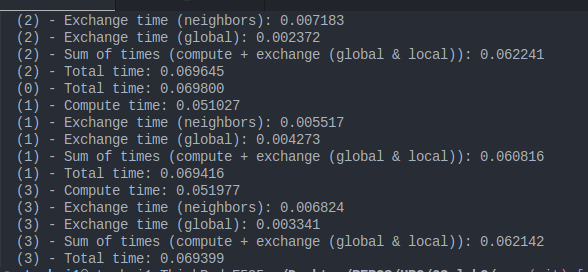
\includegraphics[width=0.7\textwidth]{../fig/lab2/ex2.png}
    \caption{Timing for the different sections.\\
    (x) \dots denotes the process rank\\
    Exchange time (neighbors) \dots time spent in \texttt{}}
    \label{fig:timing2}
\end{figure}
